%We now formally define the problem statement and the Domain Specific Language (DSL).

%\subsection{Problem Formulation}
%\label{sec-problem}

In this section we will describe 
\begin{itemize}
    \item Basic concepts of the stock bar and pattern and describe why it is hard to get the features.
    \item Why we use NN in detecting stock pattern. 
\end{itemize} 

\begin{figure}[htpb]
\begin{center}
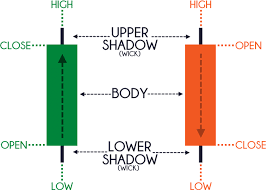
\includegraphics[width=0.4\textwidth]{./figs/candlestick}
\vspace{-0.2cm}
\caption{Stock bar for any timeframe \cite{chartpattern}}
\label{fig_bar}
\end{center}
\vspace{-0.4cm}
\end{figure}

\subsection{Stock series data}
A 'tick' is defined as a single movement in price at any given time frame. As it is very difficult and expensive to collect the tick data history, we used data with larger timeframes in our experiments. A candle bar is commonly used to depict price movement behaviors in a unit timeframe. A bar has 4 data points. Open, high, low, close, as shown in Figure \ref{fig_bar}.

\subsection{Chart pattern}
When seen in multiple timeframes, stock prices follow different chart patterns that indicate certain future price movements with high likelihoods. Before the advent of machine learning in finance, statisticians made predictions by recognizing these patterns. Some of the well known examples of chart patterns are given in figure \ref{fig_pattern}. Since they are not always easily detected with bared eyes, we are motivated to use NN to detect the patterns. As NN is known to capture fuzzy features from large datasets, we can conclude that NN can also predict results with empirical evidence from the past price movements such as these patterns. 


\begin{figure}[htpb]
\begin{center}
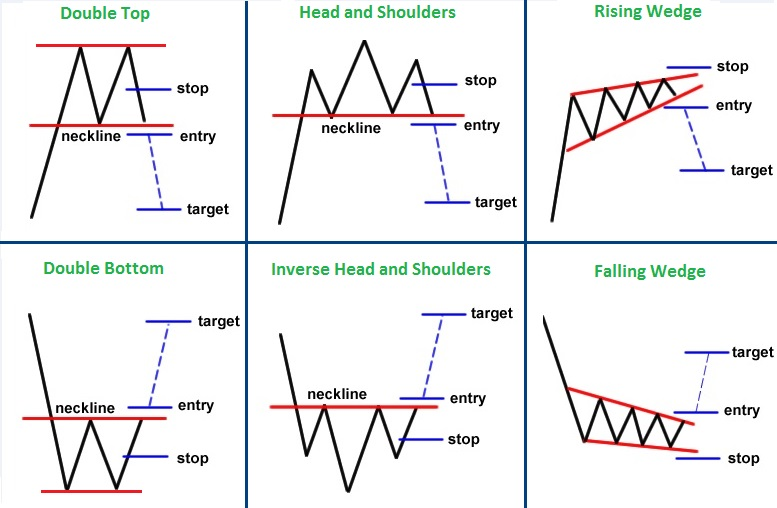
\includegraphics[width=0.9\textwidth]{./figs/chart-patterns}
\vspace{-0.2cm}
\caption{Different stock pattern across timestep \cite{chartpattern}}
\label{fig_pattern}
\end{center}
\vspace{-0.4cm}
\end{figure}



